\section{Hasil}

\begin{frame}
\frametitle{Hasil  algoritma genetika dengan banyak klaster berbeda}
\begin{block}{Total jarak dari tiap pembagian klaster}
\begin{table}[H]
\centering
\footnotesize
\begin{tabular}{ccccc}
\rowcolor[HTML]{4472C4} 
\cellcolor[HTML]{4472C4}{\color[HTML]{FFFFFF} } &
  \cellcolor[HTML]{4472C4}{\color[HTML]{FFFFFF} } &
  \cellcolor[HTML]{4472C4}{\color[HTML]{FFFFFF} } &
  \multicolumn{2}{c}{\cellcolor[HTML]{4472C4}{\color[HTML]{FFFFFF} \textbf{Titik Asal}}} \\
\rowcolor[HTML]{4472C4} 
\multirow{-2}{*}{\cellcolor[HTML]{4472C4}{\color[HTML]{FFFFFF} \textbf{Banyak Klaster}}} &
  \multirow{-2}{*}{\cellcolor[HTML]{4472C4}{\color[HTML]{FFFFFF} \textbf{Total Jarak}}} &
  \multirow{-2}{*}{\cellcolor[HTML]{4472C4}{\color[HTML]{FFFFFF} \textbf{Peringkat}}} &
  \cellcolor[HTML]{4472C4}{\color[HTML]{FFFFFF} \textbf{Latitude (X)}} &
  \cellcolor[HTML]{4472C4}{\color[HTML]{FFFFFF} \textbf{Longitude (Y)}} \\
\onslide<2-> 1  & 10,0503  & 10 & -7,8221841 & 113,3570412 \onslide<3-> \\
\rowcolor[HTML]{D9E1F2} 
2  & 6,858777 & 9  & -7,8241236 & 113,3236903 \onslide<4-> \\
3  & 5,599878 & 8  & -7,8219762 & 113,3512877 \onslide<5->\\
\rowcolor[HTML]{D9E1F2} 
4  & 5,010994 & 7  & -7,8215022 & 113,3644199 \onslide<6-> \\
5  & 4,805015 & 6  & -7,828521  & 113,3744846 \onslide<7-> \\
\rowcolor[HTML]{D9E1F2} 
6  & 4,43132  & 3  & -7,8265701 & 113,3475373 \onslide<8-> \\
7  & 4,353295 & 1  & -7,8331118 & 113,3721289 \onslide<9-> \\
\rowcolor[HTML]{D9E1F2} 
8  & 4,398984 & 2  & -7,8358502 & 113,3704048 \onslide<10-> \\
9  & 4,48243  & 4  & -7,8321462 & 113,356253  \onslide<11-> \\
\rowcolor[HTML]{D9E1F2} 
10 & 4,780413 & 5  & -7,8406976 & 113,3665328
\end{tabular}
\end{table}
\end{block}
\end{frame}

\begin{frame}
\frametitle{Hasil algoritma genetika dengan banyak klaster berbeda}
	\begin{figure}
	\centering
		\begin{subfigure}[h]{0.2\textwidth}
		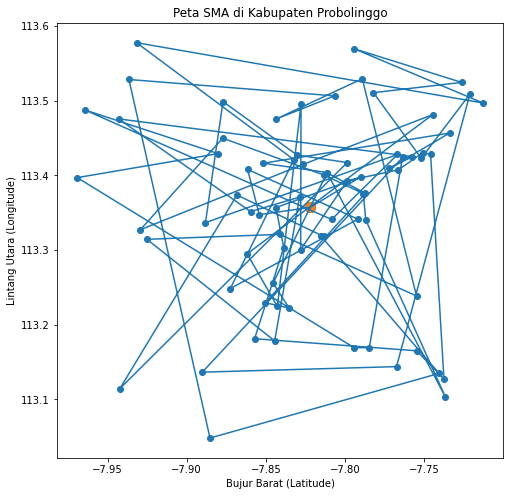
\includegraphics[width=\textwidth]{gambar/hasil_mtsp/1}
		\caption{Tanpa klaster}
		\end{subfigure}
		\hfill
		\begin{subfigure}[h]{0.2\textwidth}
		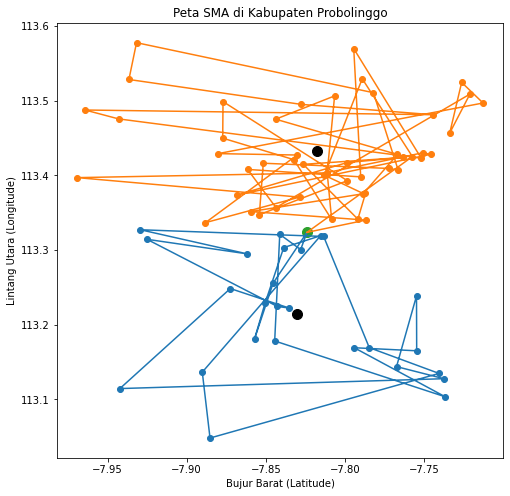
\includegraphics[width=\textwidth]{gambar/hasil_mtsp/2}
		\caption{2 klaster}
		\end{subfigure}
		\hfill
		\begin{subfigure}[h]{0.2\textwidth}
		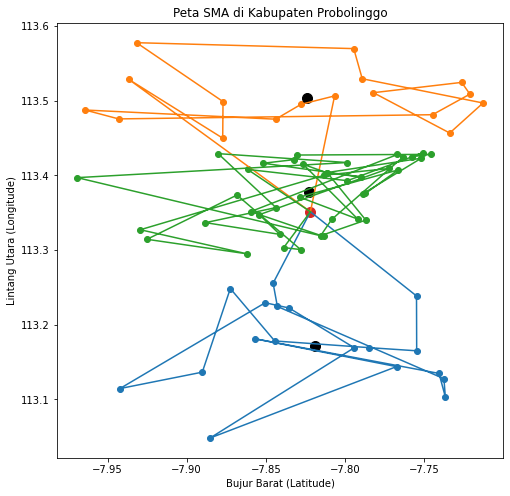
\includegraphics[width=\textwidth]{gambar/hasil_mtsp/3}
		\caption{3 klaster}
		\end{subfigure}
		\hfill
		\begin{subfigure}[h]{0.2\textwidth}
		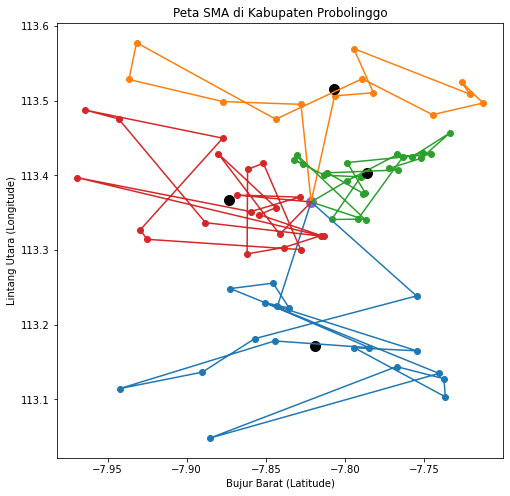
\includegraphics[width=\textwidth]{gambar/hasil_mtsp/4}
		\caption{4 klaster}
		\end{subfigure}
		\hfill
		\begin{subfigure}[h]{0.2\textwidth}
		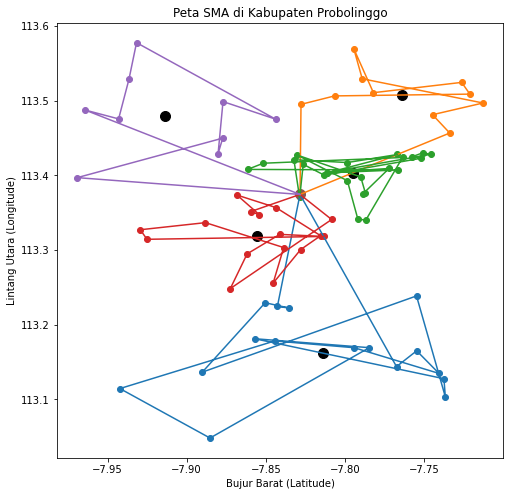
\includegraphics[width=\textwidth]{gambar/hasil_mtsp/5}
		\caption{5 klaster}
		\end{subfigure}
		\hfill
		\begin{subfigure}[h]{0.2\textwidth}
		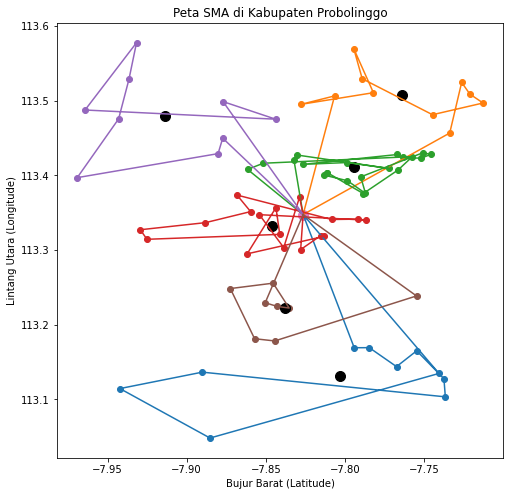
\includegraphics[width=\textwidth]{gambar/hasil_mtsp/6}
		\caption{6 klaster}
		\end{subfigure}
		\hfill
		\begin{subfigure}[h]{0.2\textwidth}
		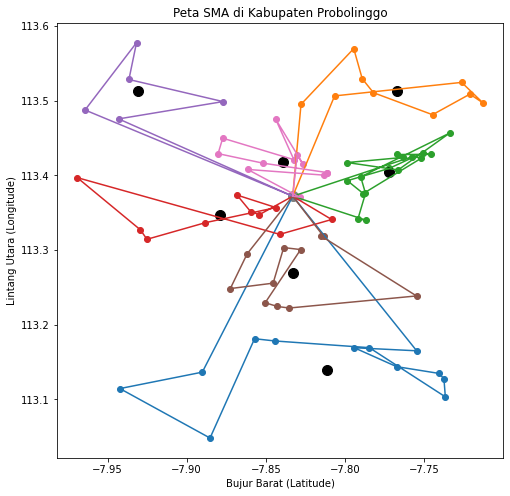
\includegraphics[width=\textwidth]{gambar/hasil_mtsp/7}
		\caption{7 klaster}
		\end{subfigure}
		\hfill
		\begin{subfigure}[h]{0.2\textwidth}
		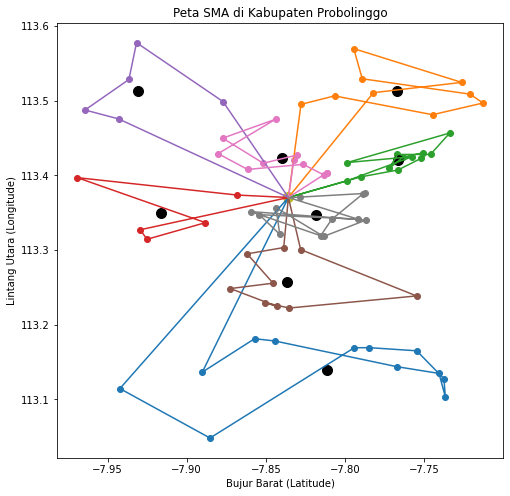
\includegraphics[width=\textwidth]{gambar/hasil_mtsp/8}
		\caption{8 klaster}
		\end{subfigure}
	\end{figure}
\end{frame}